%%%%%%%%%%%%%%%%%%%%%%%%%%%%%%%%%%%%%%%%%%%%%%%%%%%%%%%%%%%%%%%%%%%%%%
% Slides
%%%%%%%%%%%%%%%%%%%%%%%%%%%%%%%%%%%%%%%%%%%%%%%%%%%%%%%%%%%%%%%%%%%%%%

\begin{frame}
\titlepage
\end{frame}

\begin{frame}{Overview}
  \tableofcontents
\end{frame}

\section{Introdução}

\begin{frame}{Exemplo de slide com figura}
  \begin{columns}
    \column{0.5\textwidth}
    \begin{itemize}
    \item Escreva frases curtas! =)
    \end{itemize}

    \column{0.5\textwidth}
    \begin{figure}
      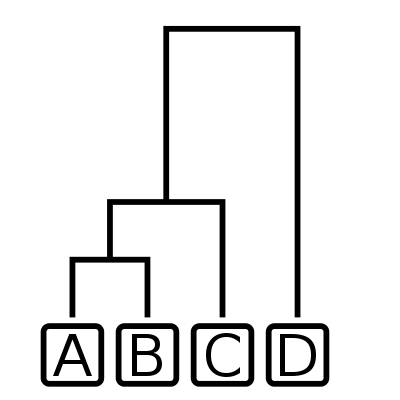
\includegraphics[width=\textwidth]{example}
      \caption{Legenda da figura.}
      \label{fig:exemplo}
    \end{figure}
  \end{columns}
\end{frame}

\section{Conclusão}

\begin{frame}{Exemplo de slide com blocos}
  \begin{block}{Hipótese}
    Não existe...
  \end{block}

  \begin{block}{Objetivos}
    \begin{itemize}
    \item Fazer isso.
    \item Fazer aquilo.
    \end{itemize}
  \end{block}
\end{frame}

\appendix

\begin{frame}
  \frametitle{Obrigado pela atenção!}
  \begin{center}
    {\Huge Obrigado!}
  \end{center}
\end{frame}

\begin{frame}[allowframebreaks]
  \frametitle{Créditos}
  \begin{description}
  \item[Slide~\pageref{fig:exemplo}]
    \url{http://hackage.haskell.org/package/hierarchical-clustering-diagrams}.
  \end{description}
\end{frame}
